\chapter{Neurónová sieť}\label{chap:neuralnet}

Keďže \textit{umelá neurónová sieť} je významnou časťou tejto práce, venujeme jej samostatnú kapitolu. Popíšeme rôzne architektúry sietí, ktoré sme vyskúšali a porovnáme ich vlastnosti a úspešnosť pri riešení problému rozpoznania ruky.

\section{Cieľ}

Našim cieľom je vytvoriť vhodnú architektúru neuónovej siete, ktorá bude rozhodovať o danom vstupe, či zodpovedá ruke alebo nie. Vyskúšame niekoľko typov architektúr, porovnáme ich a následne vyberieme najvhodnejšiu, ktorú potom použijeme. 

Neurónová sieť má rozdeliť vstupy do 2 tried - tie, ktoré zodpovedajú rukám a ostatné. Na to využijeme vo všetkých architektúrach jeden výstupný neurón.

\section{Jednoduchý spojitý perceprtón}

\textbf{Jednoduchý spojitý perceprtón} je základnou jednotkou našich neurónových sietí a plní úlohu neurónu. Aktivačnou funkciou je sigmoida: $f(x) = \frac{1}{1+e^{-x}}$, kde $x$ je váhovaná suma vstupov. Viac o neurónových sieťach môžete nájsť napríklad v \cite{haykin1999neural}. 

Takýto perceptrón robí zobrazenie $\mathbb{R}^n\rightarrow (0,1)$, kde $n$ je rozmer vstupu.

\section{Vrstva neurónovej siete}

\textbf{Vrstva neurónovej siete} sa skladá z niekoľkých jednoduchých spojitých perceptrónov (neurónov). Každý neurón sa aktivuje samostatne - nezávisle od ostatných.

Vrstva robí zobrazenie $\mathbb{R}^n\rightarrow (0,1)^m$, kde $n$ je rozmer vstupu a $m$ je počet neurónov vo vrstve.

\section{Viac vrstvová dopredná neurónová sieť}

\begin{wrapfigure}{r}{0.4\textwidth}
  \begin{center}
    \includegraphics[width=0.3\textwidth]{images/ffnn}
  \end{center}
  \caption{Dopredná neurónová sieť}
  \label{fig:ffnn}
  \begin{center}
    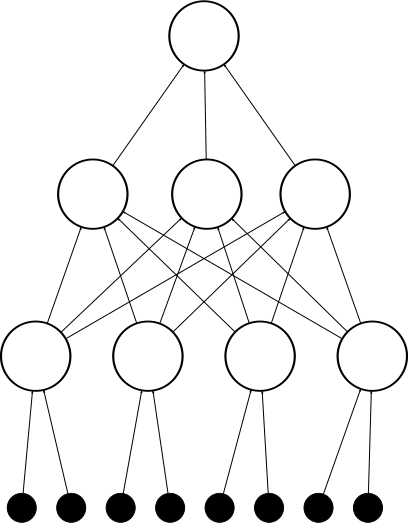
\includegraphics[width=0.3\textwidth]{images/dffnn}
  \end{center}
  \caption{Upravená dopredná neurónová sieť}
  \label{fig:dffnn}
\end{wrapfigure}


\textbf{Viac vrstvová dopredná neurónová sieť} (obr. \ref{fig:ffnn}) je neurónová sieť zložená z viacerých vrstiev neurónov, pričom signál sa šíri len zo spodnejšej vrstve na vyššiu. V našej implementácii siete sa ako vstup každého neurónu berie výstup každého neurónu z predošlej vrstvy. Prvá vrstva dostane pôvodný vstup. 

\section{Viac vrstvová dopredná neurónová sieť - upravená verzia}

V upravenej verzii sme upravili spodnú vrstvu siete - tú, ktorá dostáva vstup. Vstup je rozdelený na 16 častí a ku každej časti je pridelených niekoľko neurónov. Každý neurón spracúva len vstupy z jeho časti (obr. \ref{fig:dffnn}). 

Jej výhodou je rýchlosť. Náš vstup má rozmer $128\times 128 = 16384$, čo nie je malé číslo. Rozdelíme ho na 16 častí s veľkosťou $32\times 32 = 1024$. Takto namiesto toho aby každý vstupný neurón počítal s 16384 vstupmi počíta len s 1024, čo je $16\times$ rýchlejšie. Skupina neurónou pridelená danej časti sa stará len o príznaky zo svojej časti a nie je ovplyvňovaná ostatnými časťami. 

Nevýhodou je to, že neuróny sú fixne pridelené na jednotlivé vstupy. V pôvodnej sieti si neuróny sami vyberali, ktoré časti vstupu sú pre nich najvýznamnejšie a mohli tak lepšie pokryť vstup.
